% !TEX root = Paper.tex
\IEEEPARstart{T}{he} increasing penetration of renewable energy sources in the electrical grid has led to a significant rise in the use of power electronic converters. These converters are essential for integrating RES into the grid, as they facilitate the conversion of DC power generated by sources like solar panels and wind turbines into AC power compatible with the grid. However, the widespread use of power electronic converters has also introduced challenges related to power quality, such as the injection of harmonics and non-linear loads, which can lead to voltage distortions and other issues in the electrical grid.

There are many solutions that have been proposed to address the power quality issues in the grid, such as STATCOMs, the dynamic voltage restorers (DVRs) active power filters (APFs), the unified power quality conditioners (UPQC) and the solid-state transformers (SST). SSTs has the ability to mitigate most of the power quality issues mentioned above, while also providing galvanic isolation and voltage transformation. However, the high cost and complexity of SSTs has limited their widespread adoption in the distribution grid and, also, does not provide the same short-circuit current capability as traditional distribution transformers (DTs).

\begin{figure*}[t!]
    \centering
    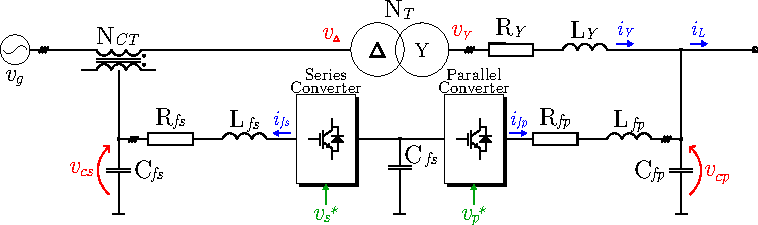
\includegraphics[width=0.9\textwidth]{Images/HDT_Diagram.pdf} 
    \caption{Hybrid distribution transformer circuit diagram.}
    \label{fig:HDT_Transformer}
\end{figure*}

For this reason, the hybrid distribution transformer (HDT) emerges as a promising solution to address the disadvantages of SSTs while still providing advanced power quality functionalities.
The HDT is a power electronic transformer that combines the functions of a traditional distribution transformer with those of power electronic converters. Many HDT configurations have been proposed in the literature, and in consequence, classifications have been made~\cite{carrenoConfigurationsPowerTopologies2021}. One of the classifications is based on the source of the converter's energy, i.e., whether the energy is obtained from a capacitor/battery, the primary or secondary side of the DT, or an auxiliary winding. On the other hand, the other classification is based on how the converters inject energy into the system, i.e., whether they are connected in series or in parallel with the DT. 

In this paper, the configuration of the HDT consists of the DT connected to two back-to-back voltage source converters (VSCs): a series converter connected to the primary of the DT through a coupling transformer (CT), and a parallel converter connected in parallel to the load, which is connected to the secondary of the DT. A circuit diagram of the HDT is shown in \cref{fig:HDT_Transformer}. The series converter is responsible for regulating the voltage at the primary side of the DT, while the parallel converter is responsible for regulating the current injected into the load.

Several control strategies have been proposed for the HDT in the literature, including finite control set model predictive control (FC-MPC)~\cite{costaFourlegMatrixConverter2022}, switching V-f and P-Q mode control~\cite{xuThreePhaseHybridTransformer2023}, and decoupled control strategies, such as the resonant control~\cite{matelskiBadaniaEksperymentalneTransformatora2023} the compound controller~\cite{liuCompoundControlSystem2020}, quasi-proportional controller~\cite{liuQuasiProportionalResonantControlHybrid2022} and the separated state-feedback controller~\cite{carrenoStateFeedbackControlHybrid2024}.

In this paper, a unified control strategy based on state feedback control with resonant states is proposed for the HDT. This control strategy aims to achieve zero steady-state error for sinusoidal references and disturbances, while also ensuring good dynamic performance. The control strategy is designed using an augmented state-space model of the HDT that includes the delays introduced by the digital control system and the resonant states to achieve zero steady-state error for sinusoidal references and disturbances. The control gains are optimized using particle swarm optimization (PSO) to minimize a cost function that considers both the transient and steady-state performance of the HDT. The proposed control strategy is validated through simulation results that demonstrate its effectiveness in regulating the voltage and current of the HDT under various operating conditions.